\subsection{fulibWorkflows Web-Editor Backend}\label{subsec:backend}
Das folgende Kapitel beschäftigt sich mit dem zweiten Bestandteil des Web-Editors, das dazugehörige Backend.
Vom Frontend wird eine YAML-Beschreibung ans Backend geschickt, in diesem wird dies als Eingabe für fulibWorkflows verwendet.
Da fulibWorkflows eine Java-Bibliothek ist, benötigt es ein Backend basierend auf Java.

\subsubsection{Spring Boot}
\todo{Allgemeines}

\todo{Spring Initalizr}

Generieren grundlegendes Projekt durch Spring Initializr.\cite*{sbinit}
Sie sehen das ganze in~\ref{fig:spring-init}.

\begin{figure}[h]
    \centering
    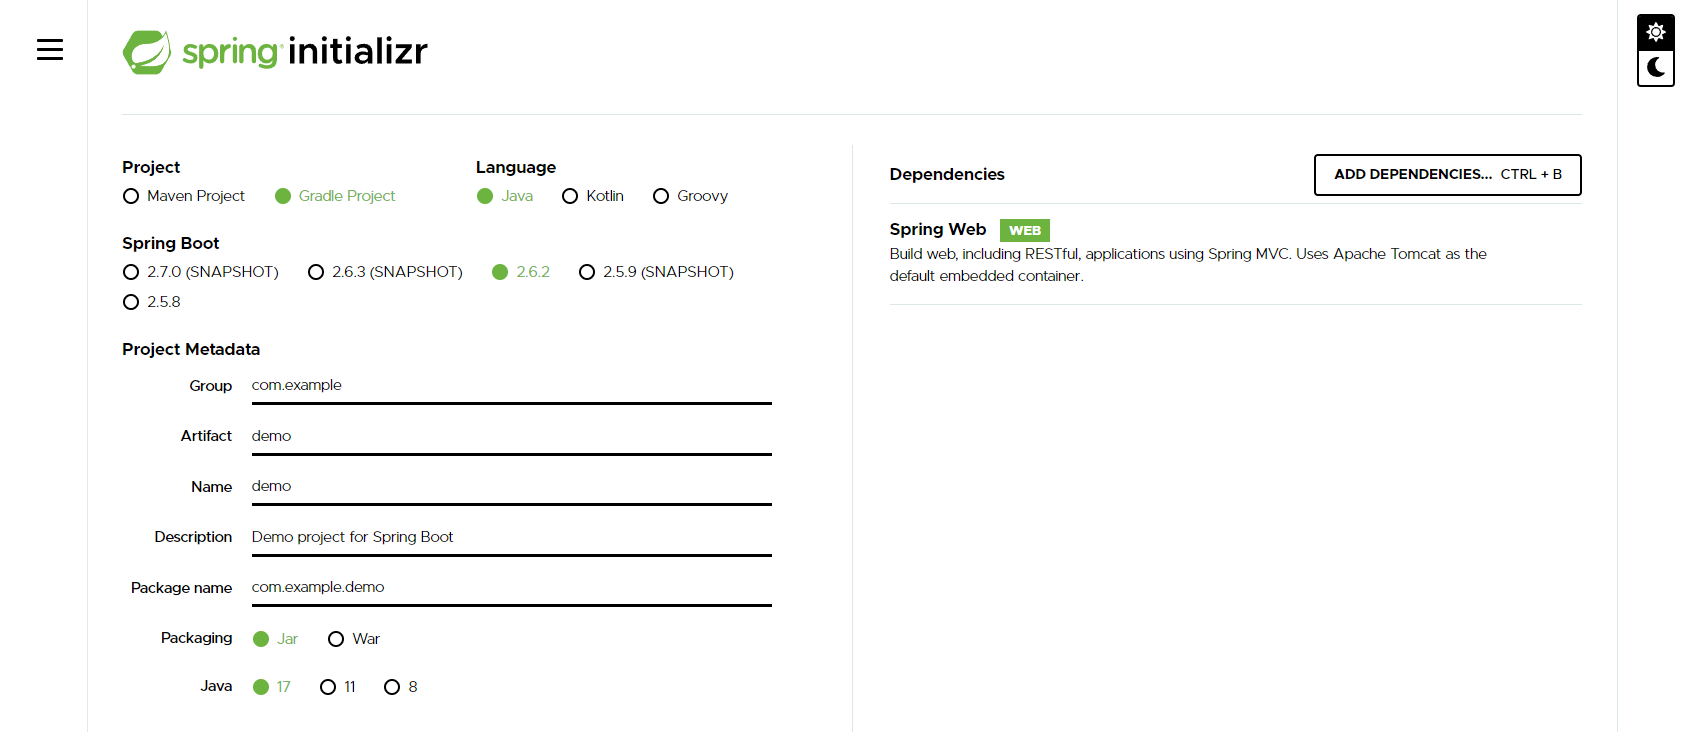
\includegraphics[width=1.0\textwidth]{images/2.2/spring-init}
    \caption{Spring Initalizr für eine Web Anwendung}
    \label{fig:spring-init}
\end{figure}


\todo{Warum Spring Boot und nichts anderes?}


Framework mit dem man easy mal ein backend generiert bekommt.
Durch Java und viele Dependency allerdings alles andere als ein leichtgewicht.

Dennoch musste ein Java backend her, da sonst fulibWorkflows nicht hätte integriert werden können.
Jedenfalls nicht ohne noch mehr middle ware.

Zudem hatte ich im Praktikum mit Spring Boot Erfahrungen gesammelt.
Die Verwendung von Annotations und dem aufsplitten zwischen Controller und Service ist mir bereits
durch Nest.js bekannt gewesen.

Dennoch muss man sagen, dass durch die von Spring Boot bereits integrierten libraries nichts weiter
außer fulibWorkflows hinzugefügt werden musste.
Immerhin umfasst der Code vom Backend vielleicht 300 Lines of Code.
